

Some patterns in the results deserve closer attention because they either sharpen the
main conclusions or serve as cautionary notes for practitioners.\\[1mm]
{\bf Adapter family determines how urgently the SAE needs retraining.}
\label{sec:obs:adapter}
LoRA modifies model weights directly, rotating and scaling the representation space in the layers it touches. As a result, it behaves as a more stable finetuning method. MaPLe and TAP leave backbone weights frozen and learn only prompt tokens that steer activations at inference time. Table~\ref{tab:clip_maple_tap_sae1} shows that LoRA is a more stable adapter, with its accuracy being affected less when using the Generic SAE compared to MaPLe and TAP. This suggests prompt-based adaptors need finetuned SAE to recover the lost accuracy.
%\vspace{-6pt}

\begin{figure}[hbt]
\centering
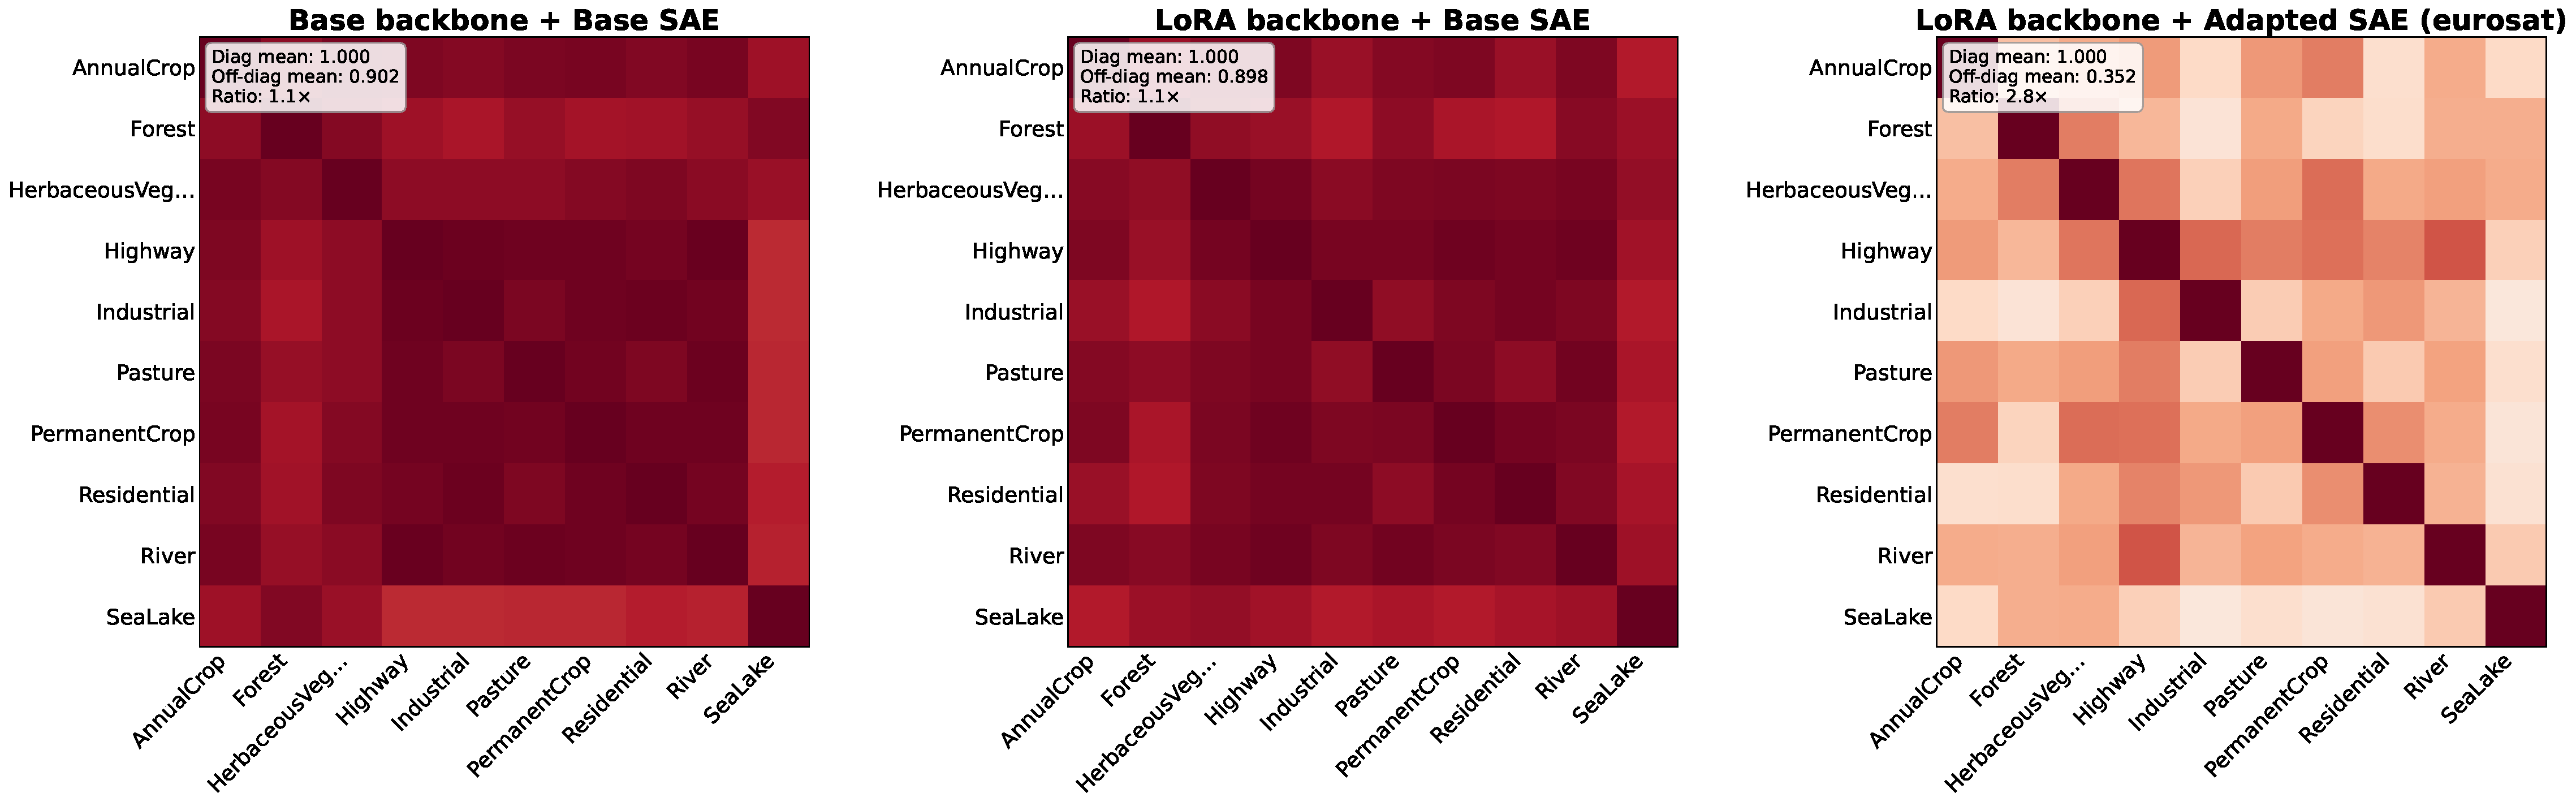
\includegraphics[width=0.9\columnwidth]{figures/class_similarity_eurosat.pdf}

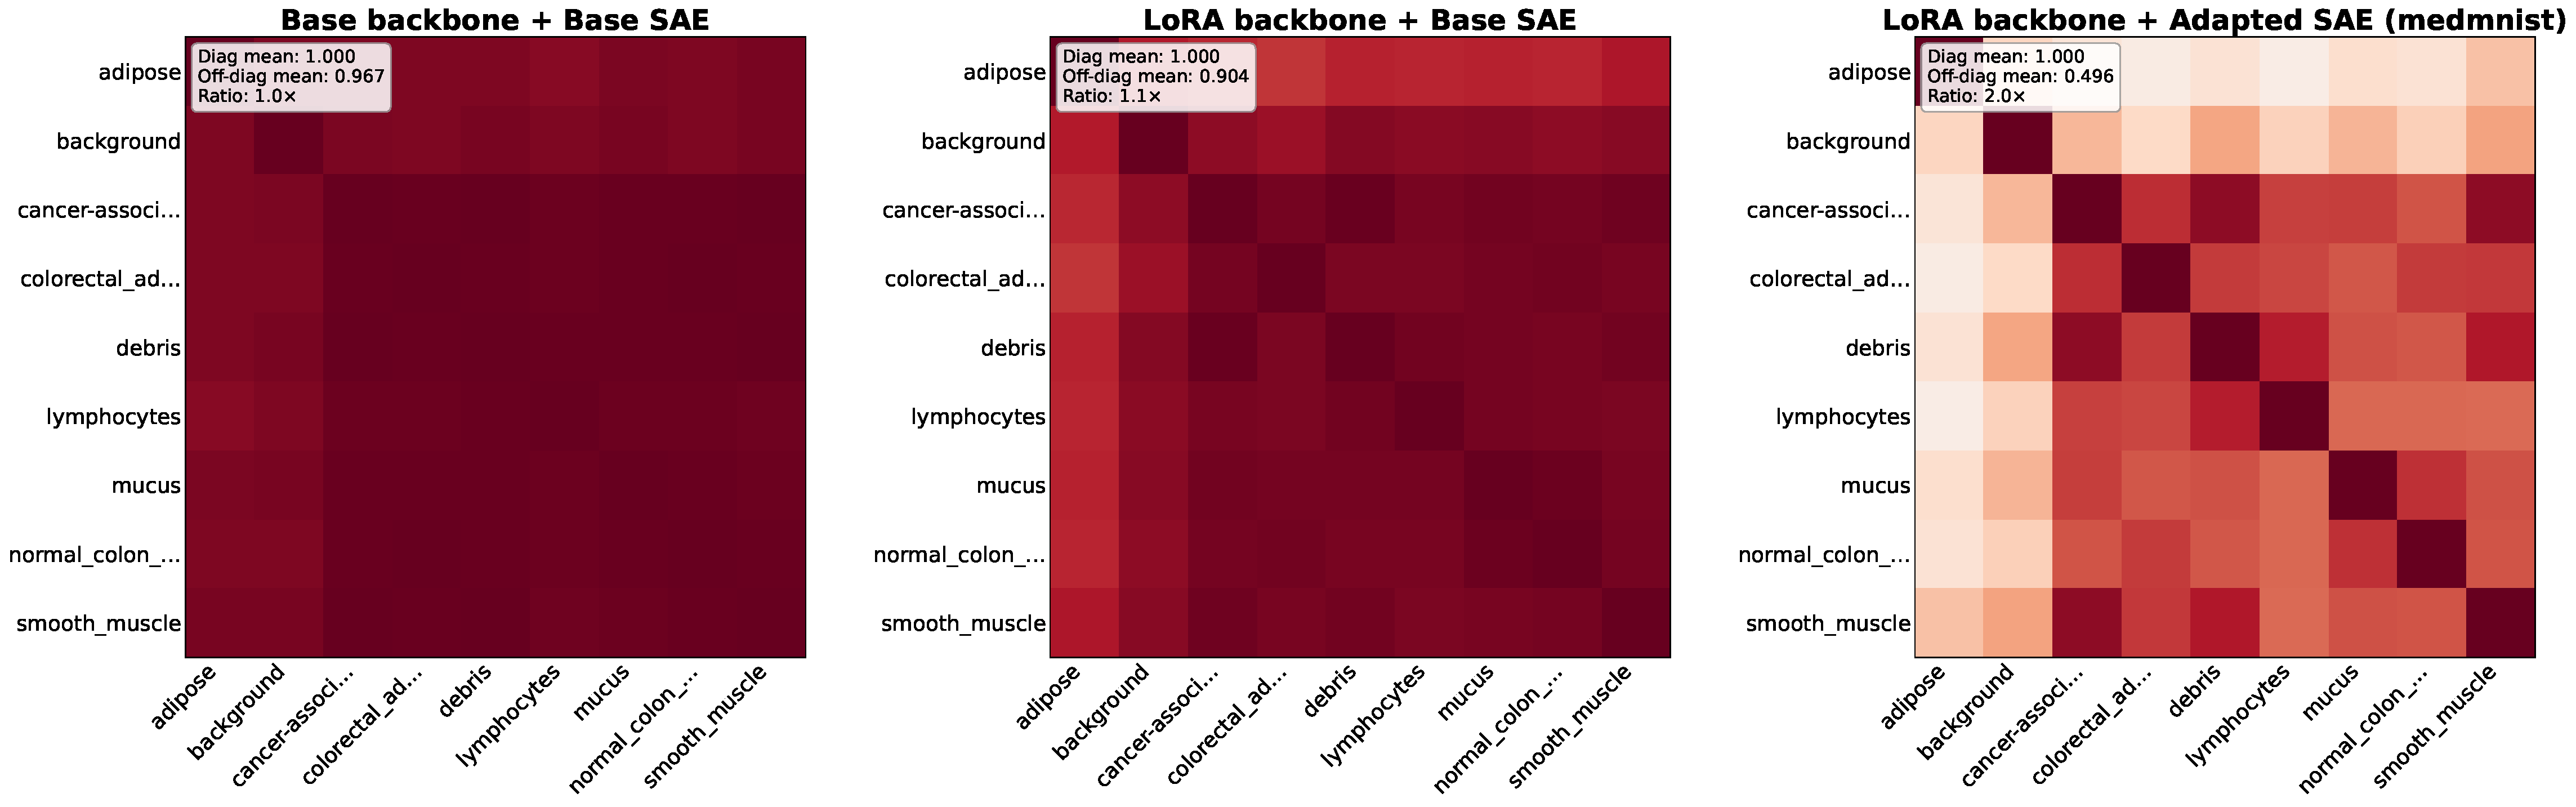
\includegraphics[width=0.9\columnwidth]{figures/class_similarity_medmnist.pdf}

%\vspace{0.9em}
%\vspace{0.4em}
\caption{Heat map of cosine similarity of top activating neurons averaged for each class. Top row: EuroSAT, bottom: PathMNIST. Left col: ZS+G-SAE, middle: FT+G-SAE, right: FT+FT-SAE. Finetuned SAEs learn more class discriminative features.}\vspace{-3mm}
\label{fig:heatmap}
\vspace{-10pt}
\end{figure}

{\bf Language supervision is required for SAE decomposability on far-domain data.}
\label{sec:obs:dino}
DINOv2, the only backbone trained without language signal, tracks the three
language-supervised models except on PathMNIST. DINOv2's
FT-SAE has low cosine similarity, high NMSE, and increased $L_0$ compared to CLIP, SigLIP, and ALIGN (Table \ref{tab:h2_metrics}).
Language-supervised training builds a feature space whose
principal directions align with semantic categories, making sparse decomposition tractable.
DINOv2's features, optimised for spatial correspondence via self-distillation, lack this
alignment on medical data where the visual vocabulary shares almost no overlap with
natural-scene statistics. SAE-based interpretability of self-supervised encoders on
far-OOD domains may be structurally out of reach without additional language-grounding.

\comment{
\vspace{-6pt}
{\bf High dead-neuron fraction can signal productive specialisation, not failure.}
The conventional reading of high dead-neuron fraction is wasted capacity. The EuroSAT
results show this can be wrong. For CLIP, the FT-SAE has $81\%$ dead neurons versus
$16\%$ for the generic SAE, yet classification accuracy is $4.5$\,pp higher (H1), $L_0$
drops from $125$ to $15$ (H2), and CosSim rises by $0.105$. The dead-neuron count here
reflects \emph{hyper-specialisation}: the adapted model encodes satellite-specific features
along a small number of directions, and the FT-SAE finds them efficiently.
Practitioners should read dead-neuron fraction alongside $L_0$ and reconstruction fidelity;
high dead fraction combined with low $L_0$ and high CosSim indicates productive
specialisation, not dictionary collapse.
}

\comment{
\vspace{-6pt}
{\bf Cosine similarity with the base feature space is not a reliable proxy
for downstream utility under large domain shift.}
\label{sec:obs:cossim}
Our CLIP PathMNIST result breaks the common assumption that reconstruction fidelity is a
good proxy for SAE utility. The FT-SAE achieves \emph{lower} CosSim than the generic
SAE ($0.730$ vs.\,$0.882$) and higher NMSE ($0.085$ vs.\,$0.035$), yet yields $3.5$\,pp
better classification accuracy (H1). The FT-SAE has learned directions nearly
orthogonal to the pretraining basis that are the correct directions for the target domain.
CosSim and NMSE should therefore be measured against the \emph{adapted} model's activations,
not the base model's. Using base-model reconstruction fidelity as a quality signal on a
shifted distribution will reliably underrate the FT-SAE and overrate the generic one.
}

{\bf Findings are robust to SAE architecture, backbone, and adaptation method.}
Our observations on the Generic SAE degrading and the Finetuned SAE recapturing performance work across SAE architectures as well as across adapters and models.
Tables \ref{tab:main_accuracy_abs}, \ref{tab:accuracy_sae2}, \ref{tab:accuracy_sae3}, and \ref{tab:accuracy_sae4} clearly show this.
To test that the procedure itself is not specific to the CLIP\,+\,LoRA\,+\,ReLU configuration the main results use, we ran the full pipeline over a wider matrix: three further encoders (DINOv2, which has no text tower at all; ALIGN, whose convolutional vision tower emits no token sequence; and SigLIP2), two further SAE architectures (Top-$k$~\citep{gao2025scaling} and JumpReLU~\citep{rajamanoharan2024jumprelu}), and two further adaptation methods (MaPLe~\citep{khattak2023maple} and VPT-Deep~\citep{jia2022visual}).
Masked finetuning runs unchanged across every combination, and unit protection is exact --- including for JumpReLU's learned per-unit threshold, which must be masked alongside the encoder and decoder weights or the units the method exists to preserve are silently modified.
Appendix~\ref{app:generality} reports the matrix, along with the two structural limits it exposes: MaPLe reaches CLIP alone because its deep visual prompts are coupled to a paired text tower, while VPT is the only method here that reaches a vision-only encoder.

{\bf Domain distance predicts degradation, but not the distance one would first reach for.}
The correlation between embedding-space $\mathrm{MMD}^2$ and generic-SAE degradation does not survive extending the cohort from six domains to eight: apparent $R^2$ falls to $0.004$, driven by a single domain (Oxford~Pets) that is stylistically the most distant in the cohort yet degrades least.
The resolution is that embedding distance conflates how different a domain's images \emph{look} with how different its concepts are from those the dictionary was fit on --- and ImageNet-1k already covers Oxford~Pets' vocabulary almost completely.
Measuring concept distance directly, as the mean cosine distance from each target class name to its nearest ImageNet-1k class name in CLIP text-embedding space, recovers a strong relationship ($\rho = 0.95$, leave-one-domain-out $R^2 = 0.506$ where the MMD fit is negative).
Combining the two yields a rule that calls retrain-versus-reuse correctly in $7$ of $8$ domains out-of-sample, using only quantities measurable before any SAE is trained.
Appendix~\ref{app:when-to-retrain} gives the fit, the model-selection procedure, and the reasons this should be read as a candidate rule rather than a validated instrument.

{\bf The generic dictionary is not merely a worse description --- it is not causally load-bearing.}
Accuracy, reconstruction fidelity and entropy are all correlational, and are equally consistent with the generic SAE being a slightly poorer but still faithful account of the adapted model.
Intervening directly on latents rules that reading out.
Using an error-preserving edit for which an unmodified latent is an exact no-op, ablating or amplifying a generic-SAE latent on the adapted model produces an effect whose confidence interval covers zero in every condition tested, indistinguishable from editing a random activity-matched latent; the finetuned SAE's latents produce far larger effects in every condition.
Extending this to multi-latent edits, how far a dictionary's top latents are \emph{necessary} to the model's correct predictions tracks domain distance with rank correlation $1.0$, while \emph{sufficiency} under amplification shows no reliable trend --- the two should not be collapsed into a single steerability number.
Appendix~\ref{app:causal} reports both.
A separate ablation (Appendix~\ref{app:init}) isolates what the generic checkpoint itself contributes: near the pretraining distribution a scratch-trained SAE matches the finetuned one, and the initialisation only begins to pay at moderate and far distance.

{\bf Ablations:}
We explore of a different combination of hyperparameters for SAE can compensate for the loss in interpretability performance. We explored different expansion factors for the the SAE encoder layer to see if a richer SAE can preserve semantics better. Table \ref{tab:expansion_ablation} shows that a larger Generic SAE does help, but reaching the performance of FT-SAE may be a long way off. Larger SAEs also need significantly higher computations.

We also explored if training the Generic SAE on a richer base dataset can compensate for the loss in interpretability performance. Second-last row of Table \ref{tab:expansion_ablation} shows the results of training a $64\times$ SAE on the larger, CC3M dataset. The larger dataset seems to have made the performance significantly worse. This aspect needs further exploration to reach definite conclusions with our observation providing one datapoint.

{\bf Computation cost:} Training of the Generic SAE takes around 9 hours on an Nvidia RTX A6000 Ada GPU. The SAE finetuning experiments were run on a single RTX3090  and take around 6 hours to train with the specified configuration mentioned in \ref{sec:exp:setup}. VLM and DINOv2 adaptation takes around 3-5 mins.

{\bf Limitations:}
We study adaptation of popular Vision Encoders across multiple domain shifts. Due to the scope of this study, we do not do a full mechanistic analysis of effect of adaptation itself against full fine tuning of the model. Also, Unsupervised domain adaptation of CLIP models remains unexplored and the possible implications of adapting a model without any labelled data are yet to be uncovered. Our work serves as a mechanistic understanding of popular lightweight fine tuning methods and how they shape model's activation space, what methods are brittle against extreme domain shifts and how these geometries collapse with increasing distance from Imagenet. Three limits on the newer results deserve explicit statement. The retrain/reuse rule of Appendix~\ref{app:when-to-retrain} is fit on eight domains and was not pre-registered --- the concept-distance predictor was constructed after observing the anomaly it explains --- and it has not yet been scored against the domains reserved for confirmatory testing. The causal interventions of Appendix~\ref{app:causal} use a single SAE training seed per dataset, with intervals bootstrapped over evaluation examples rather than over initialisations. And the reconstruction figures in the expanded matrix of Appendix~\ref{app:generality} are training losses rather than held-out measurements, so they speak to whether the procedure runs and fits, not to how well it generalises.